%%%%%%%%%%%%%%%%%%%%%%%%%%%%%%%%%%%%%%%%%%%%%%%%%%%%%%%%%%%%%%%%%
\subsubsection{Filter}		%	TESTFÄLLE - Filter
%%%%%%%%%%%%%%%%%%%%%%%%%%%%%%%%%%%%%%%%%%%%%%%%%%%%%%%%%%%%%%%%%

\noindent
Wir werden nun das Zusammenwirken der ersten drei Phasen von \Rm genauer untersuchen. Hierbei ist der Zusammenhang zwischen einzelnen Parametern und der Güte der Filterung besonders interessant.\\[.1cm]

%	Güte der Filter, ZV
\noindent
Wir definieren nun $\Delta X=|W'|/|X|=|W'|/n$ als die Güte der Filterung. Dies entspricht dem prozentualen Verhältnis zwischen der wie in Phase 3 festgelegten Mächtigkeit der Menge $W'$ und der Mächtigkeit $n$ der Eingabemenge $X$. Wir wissen, dass die Menge $W'$ zum einen das Minimum und zum anderen kein Element der Menge $L$ enthält. Es gilt $1 \leq |W'| \leq |X|/2=n/2$ und somit $0 < \Delta X \leq 1/2$. \\[.05cm]

\noindent
Bei einer Anzahl von $rep$ Wiederholungen besitzt $\Delta X$ die absolute Häufigkeit $H_{rep}(\Delta X)= \sum_{rep} \mathbbm{1}_{\Delta X}$. Die für uns interessanten Begrifflichkeiten der \textit{relativen Häufigkeit}, des \\
\textit{(Stichproben-) Mittelwertes} und der \textit{(Stichproben-) Varianz} ergeben sich nun über:
\begin{center}
\begin{tabular}{llcl}
\textbf{Relative Häufigkeit:}&$h_{rep}(\Delta X)$& $=$& $H_{rep}(\Delta X) / rep$\\[.25cm]
\textbf{Stichprobenmittelwert:}&$\Delta\overline{X}$& $=$ & $\frac{1}{rep}\sum_{rep} \Delta X$\\[.25cm]
\textbf{Stichprobenvarianz:}&$Var[\Delta X]$ & $=$ & $\sum\limits_{i=1}^{rep} (\Delta X_i - \overline{\Delta X})^2 \cdot h_{rep}(\Delta X)$
\end{tabular}
\end{center}

\noindent
Da der Wert von $\Delta X$ von der Randomisierung der Phasen 1-3 abhängig ist, kann er als Zufallsvariable mit Wertebereich $(0,1/2]$ aufgefasst werden.\\[.05cm]


%%%%%%%%%%%%%%%%%%%%%%%%%%%%%%%%%%%%%%%%%%%%%%%%%%%%%%%%%%%%%%%%%
\noindent
\begin{minipage}[Ht]{.45\textwidth}
Führt man den Algorithmus mit gleicher Eingabe wiederholt aus, so erwartet man nach dem (schwachen) Gesetz der großen Zahlen eine resultierende Normalverteilung der Ergebnisse. Wie in Abbildung~\ref{fig: min_GgZ} zu sehen ist mit steigender Anzahl an Wiederholungen immer klarer eine glockenförmige Darstellung der Verteilung der relativen Häufigkeiten $h_{rep}(n)$ zu erkennen. Hierbei sei anzumerken, dass bei einer solchen Darstellung der visuelle Trugschluss entsteht, dass sowohl der Extrempunkt als auch die Fläche unter der vermeintlichen Kurve zu sinken scheinen.\\[.1cm]
\end{minipage}% This must go next to `\end{minipage}`
%
\hfill
%
\begin{minipage}[Ht]{.54\textwidth}
        \centering
        \vspace*{-0.5cm}
        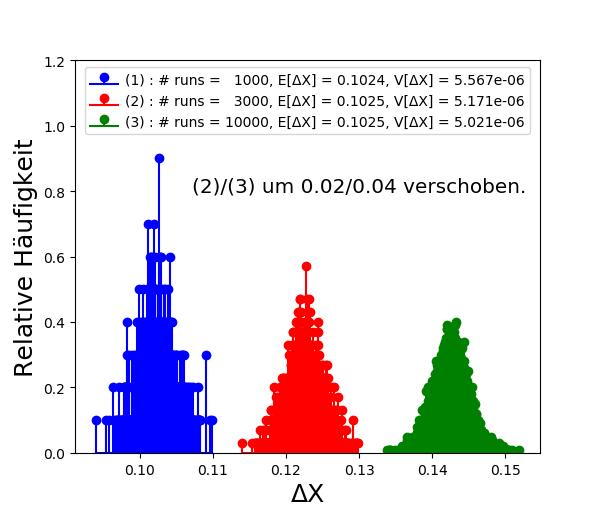
\includegraphics[scale=.66]{pictures/min_filter_runs.png}
   		\vspace*{-8mm}
   		\captionof{figure}{$\log_2(n) = 16$, $k = 64$}\label{fig: min_GgZ}

\end{minipage}

%%%%%%%%%%%%%%%%%%%%%%%%%%%%%%%%%%%%%%%%%%%%%%%%%%%%%%%%%%%%%%%%%
\noindent
Dies ist der diskreten Natur von Messwerten geschuldet. Bei einer Normalverteilung entspricht der Extrempunkt der Dichtefunktion dem Erwartungswert der zugehörigen Zufallsvariablen. Die in der Abbildung mit angegebenen Werte dienen zur Verdeutlichung der realen Entwicklung.\\[.05cm]
Von einer zugrunde liegenden Normalverteilung ausgehend wird versucht anhand der Parameter Abschätzungen für den Erwartungswert und die Varianz zu bilden.\\[.1cm]

\noindent
Um die Abhängigkeiten zu einzelnen Parametern getrennt nachzuweisen wurde für die Eingabe der Form $(n,k)$ stets einer der beiden Parameter fixiert, während für den anderen verschiedene Werte durchlaufen wurden. Dies erlaubt bestehende Korrelationen zu dem variablen Parameter zu erkennen. Für jeden hier erwähnten Fall wurden ohne anderweitige Angabe jeweils zehntausend Durchläufe ausgeführt und die Ergebnisse von $\Delta X$ separat gespeichert.\\[0.05cm]

\noindent
Im Folgenden wird die relative Häufigkeit mit $h(n)$, der Mittelwert mit $\mu$ sowie die Varianz mit $V(n,k)$ bezeichnet. Die relative Häufigkeit entspricht graphisch der Dichtefunktion der Zufallsvariable $\Delta X$.

%%%%%%%%%%%%%%%%%%%%%%%%%%%%%%%%%%%%%%%%%%%%%%%%%%%%%%%%%%%%%%%%%
%	Erwartungswert
% ---------------------------------------------------------------
%	ABHÄNGIGKEIT von N
\subsubsection*{Erwartungswert}
Nun soll die Abhängigkeit des Erwartungswertes von den Parametern $n$ und $k(n)$ untersucht werden. Hierzu wird zuerst der Parameter $k$ nacheinander auf verschiedene Werte fixiert und die Veränderung des Erwartungswertes abhängig von $n$ gemessen.\\[.1cm]
Den präsentierten Grafiken liegt die Fixierung von $k\in\{4, 32, 256\}$ für $\log_2(n)\in\{9,\cdots, 20\}$ zugrunde.

% ---------------------------------------------------------------
%	FIG: Abhängigkeit von N
\begin{figure}[H]
	%
    \hspace*{-1cm}
    \begin{minipage}[t]{.30\textwidth}
        \centering
        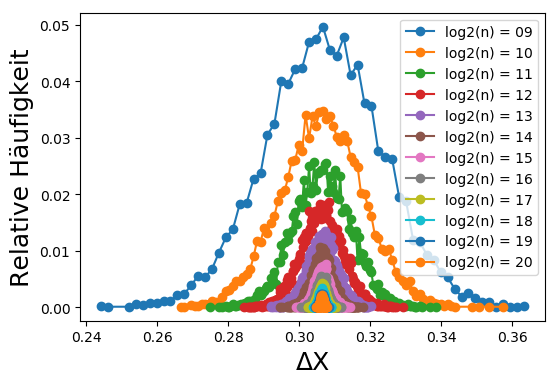
\includegraphics[width=1.2\textwidth]{pictures/min_filter_D_n_4.png}
    \end{minipage}
	%    
    \hspace*{0.8cm}
	%    
    \begin{minipage}[t]{.30\textwidth}
        \centering
        \raisebox{0.05cm}{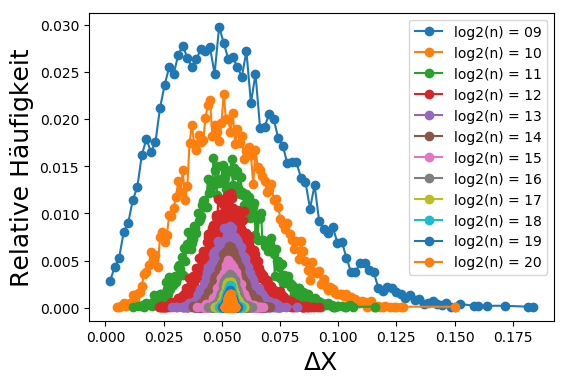
\includegraphics[width=1.21\textwidth]{pictures/min_filter_D_n_256.png}}
    \end{minipage}  
        \hspace*{0.8cm}
    \begin{minipage}[t]{.30\textwidth}
        \centering
        \raisebox{-0.05cm}{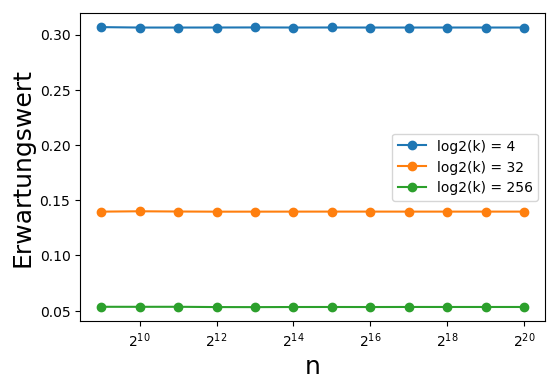
\includegraphics[width=1.2\textwidth]{pictures/min_filter_E_n}}
    \end{minipage}
    \captionof{figure}{$h(n)$ für $k=4$ und $k=256$ sowie $\mu$ für $k=4,32, 256$.}\label{fig: min_E_n}
\end{figure}

% ---------------------------------------------------------------
\noindent
Wie in Abbildung~\ref{fig: min_E_n} eindeutig zu erkennen, ist bleibt der Erwartungswert nach Fixierung von $k$ konstant für alle Werte für $n$.\\[.1cm]

% ===============================================================
%	ABHÄNGIGKEIT von K
\noindent
Nun wird der Parameter $n=2^{16}$ fixiert und alle Werte für $k=2^i$, $i\in\mN$, $k<n$ untersucht.\\

\noindent
Diesbezüglich wird sich nun auff die Aussage von Lemma~\ref{lem: min_2} berufen. Demnach gilt $\mathbb{E}[|W'_i|]\leq 2d\sqrt{k}$ für eine Konstante $d>0$. Insgesamt existieren $n/2k$ Teilmengen, womit folgt:
\[
\frac{|W'|}{|X|}=\frac{1}{n}\cdot \sum\limits_{i=1}^{n/k}\mathbb{E}[|W'_i|]=\frac{1}{n}\cdot \frac{n}{2k} \cdot \mathbb{E}[|W'|]\leq\frac{1}{2k}\cdot 2d\sqrt{k}=\frac{d}{\sqrt{k}}
\]

\noindent
Anhand der empirischen Daten wurde nun  mithilfe des Programms Gnuplot~\cite{gnu} versucht ein möglicher Fit für eine Abschätzung von $\mathbb{E}[\Delta X]$ zu berechnen.

% ---------------------------------------------------------------
%	FIG: Abhängigkeit von K
\begin{figure}[H]
    \hspace*{-0.8cm}
    \begin{minipage}[t]{.30\textwidth}
        \centering
        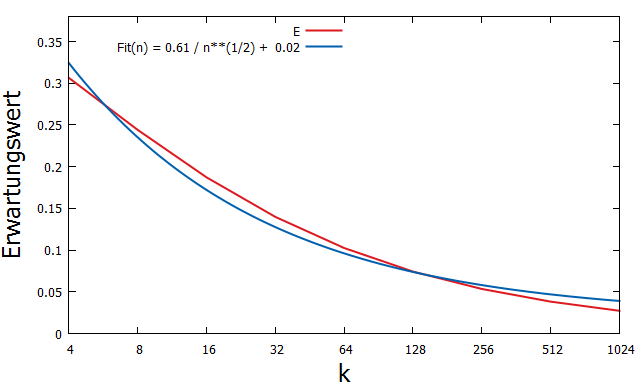
\includegraphics[width=1.2\textwidth]{pictures/min_filter_D_k.png}
    \end{minipage}
    \hspace*{.8cm}
    \begin{minipage}[t]{.30\textwidth}
        \centering
		\raisebox{-0.23cm}{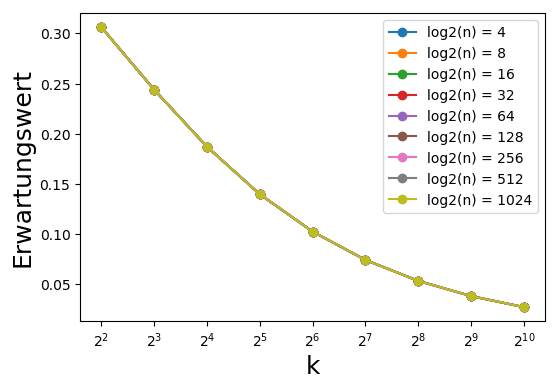
\includegraphics[width=1.1\textwidth]{pictures/min_filter_E_k.png}}
    \end{minipage}  
    \hspace*{.5cm}
    \begin{minipage}[t]{.30\textwidth}
        \centering
        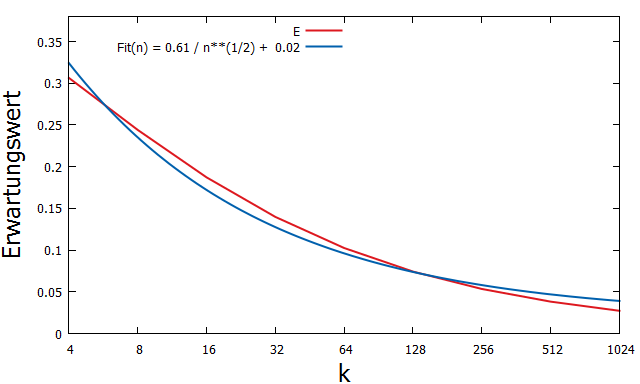
\includegraphics[width=1.2\textwidth]{pictures/min_filter_fit_E_k}
    \end{minipage}
    \captionof{figure}{$h(n)$ und $\mu$ für $\log_2(n)=16$, $\log_2(k)\in\{1,\cdots,15\}$ sowie Fit für $\mu$.}\label{fig: min_E_k}
\end{figure}

% ---------------------------------------------------------------
\noindent
Als Fit Funktion wurde hierfür $F_E(k)= a / \sqrt{k} + b$ und als Startwerte $a=0.5$ sowie $b=0.01$ gewählt. Nach 5 Iterationen ist der Fit konvergiert und die finale Summe der Residuenquadrate betrug $0.0011$. Es ergab sich eine Parametrisierung von $0.61$ und $b=0.03$. Vergleichbare Experimente ergaben ähnliche Ergebnisse, was die Aussage von Lemma~\ref{lem: min_2} bestätigt.\\[.1cm]
%%%%%%%%%%%%%%%%%%%%%%%%%%%%%%%%%%%%%%%%%%%%%%%%%%%%%%%%%%%%%%%%%
%	VARIANZ
% ---------------------------------------------------------------
%	ABHÄNGIGKEIT von N
\subsubsection*{Varianz}
Nun kann die Abhängigkeit der Varianz von den Parametern $n$ und $k(n)$ untersucht werden.\\[.1cm]
Wie schon beim Erwartungswert wird mit der Abhängigkeit von $n$ begonnen und $k$ dafür auf verschiedene Werte fixiert. Für eine direkte Vergleichbarkeit wurde für die Grafiken der gleiche Datensatz genutzt.

% ---------------------------------------------------------------
%	FIG: Abhängigkeit von N
\begin{figure}[H]
    \hspace*{-1cm}
    \begin{minipage}[t]{.30\textwidth}
        \centering
        \raisebox{-0.15cm}{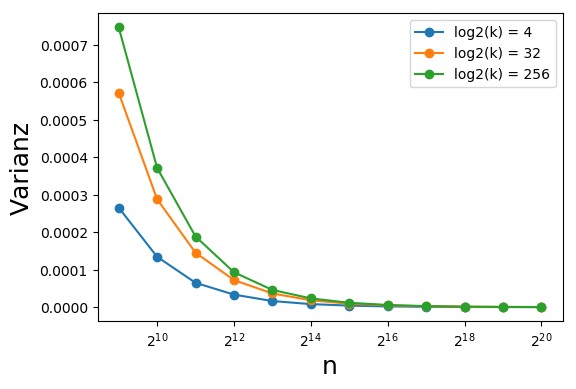
\includegraphics[width=1.1\textwidth]{pictures/min_filter_V_n.png}}
    \end{minipage}
    \hspace*{0.5cm}
    \begin{minipage}[t]{.30\textwidth}
        \centering
        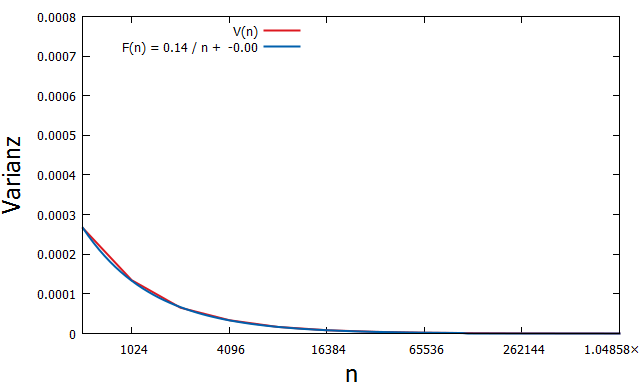
\includegraphics[width=1.2\textwidth]{pictures/min_filter_fit_V4_n.png}
    \end{minipage}  
    \hspace*{0.8cm}
    \begin{minipage}[t]{.30\textwidth}
        \centering
        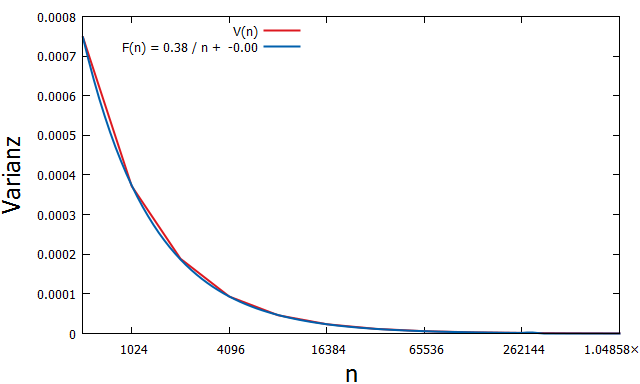
\includegraphics[width=1.21\textwidth]{pictures/min_filter_fit_V256_n.png}
        
    \end{minipage}
    \vspace*{-0.1cm}
    \captionof{figure}{$V(n)$ für $k\in\{4,32,256\}$ sowie Fit für $k\in\{4,256\}$.}\label{fig: min_V_n}
\end{figure}

% ---------------------------------------------------------------
\noindent
Wie in Abbildung~\ref{fig: min_V_n} zu sehen ähnelt der Verlauf der Varianz $V(n)$ dem einer Hyperbel. Der Fit wurde dementsprechend mit $F_V(n)=a/n + b$ mit den Startwerten $a=0.4$ und $b=0.0000001$ gewählt. Nach 5 Iterationen ist der Fit konvergiert. Die finale Summe der Residuenquadrate und weitere relevante Parameter liegen dieser Arbeit bei. Anzumerken ist hier, dass
sich die Parametrisierung von $b=0$ für alle experimentellen Werte von $k$ ergab.\\[.1cm]

\noindent
% ---------------------------------------------------------------
%	ABHÄNGIGKEIT von K
Abschließend wird noch die Abhängigkeit der Varianz $V(n,k)$ von dem Parameter $k$ geprüft und $n$ wie bereits zuvor auf $\log_2(n)=16$ fixiert.

% ---------------------------------------------------------------
%	FIG: Abhängigkeit von K
\begin{figure}[H]
    \hspace*{-1cm}
    \begin{minipage}[t]{.30\textwidth}
        \centering
        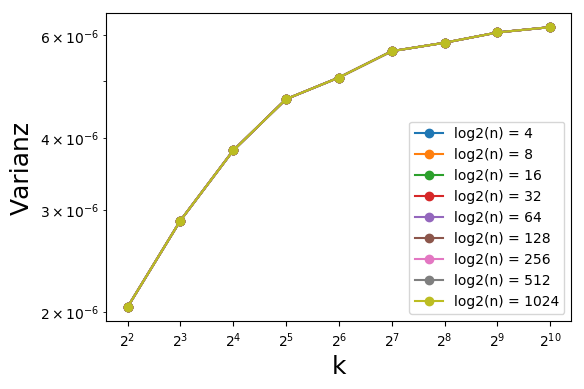
\includegraphics[width=1.2\textwidth]{pictures/min_filter_V_k.png}
    \end{minipage}
    \hspace*{.8cm}
    \begin{minipage}[t]{.30\textwidth}
        \centering
        \raisebox{0.05cm}{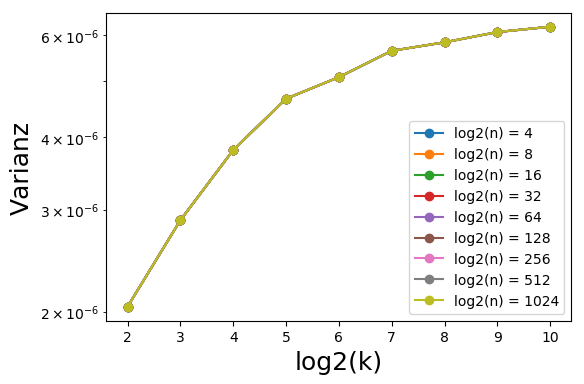
\includegraphics[width=1.21\textwidth]{pictures/min_filter_V_k_log.png}}
    \end{minipage}  
    \hspace*{.8cm}
    \begin{minipage}[t]{.30\textwidth}
        \centering
        \raisebox{0.05cm}{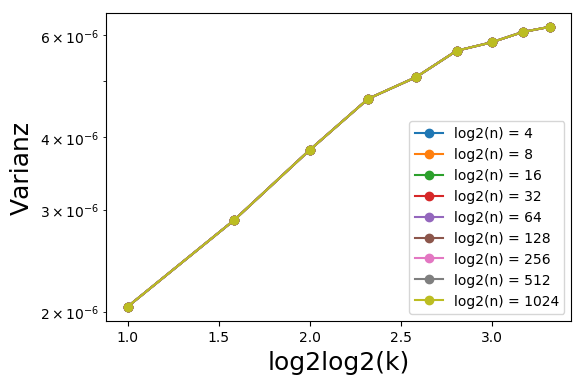
\includegraphics[width=1.21\textwidth]{pictures/min_filter_V_k_loglog.png}}
    \end{minipage}
    \vspace*{-.1cm}
    \captionof{figure}{$V(k)$ für $\log_2(n)=16$ bezüglich $k$, $\log_2(k)$ sowie $\log_2 \log_2(k)$.}\label{fig: min_V_k}
\end{figure}

% ---------------------------------------------------------------
\noindent
Da sich im Verlauf der Experimente eine logarithmischer Zusammenhang erkennen ließ, wurden wie in Abbildung~\ref{fig: min_V_k} zu sehen die Werte von $V(n)$ zuerst gegen die Werte von $k$, dann gegen die logarithmierten und abschließend gegen die doppelt-logarithmierten Werten von $k$ abgetragen. Ist bei der einfach-logarithmischen Darstellung noch eindeutig eine Kurve zu erkennen, so deutet sich bei der doppelt-logarithmischen Darstellung klar ein linearer Funktionsverlauf an.\\[.1cm]
Um sicherzustellen, dass es tatsächlich um einen doppelt-logarithmischen Zusammenhang handelt wurden nun zwei potentielle Fits in Form von $F_V^1(k)= a * \log_2(k) + b$ sowie $F_V^2(k)=a * \log_2\log_2(k) + b$ gebildet. Die nachfolgende Tabelle fasst eine um den Faktor $10^6$ skalierte Gegenüberstellung beider Fits zusammen:

\begin{center}
\begin{tabular}{c||l|l|l|l}

&\multicolumn{1}{c|}{Param $a$}&
\multicolumn{1}{c|}{Param $b$}&
\multicolumn{1}{c|}{Sum Res}&
\multicolumn{1}{c}{$\Delta$ Last Iter}\\
\hline
$F_V^1(k)$:&$0.5212$&$1.5603$&$1.3470$&$-4.6484e-14$\\
\hline
$F_V^2(k)$:&$1.9097$&$0.0636$&$0.1797$&$-9.00343e-10$

\end{tabular}
\end{center}

\noindent
An Parameter $b$ lässt sich bereits erkennen, dass $F_V^1(k)$ eine merkliche Verschiebung auf der $Y$-Achse benötigt, um eine passende Regression zu bilden. Dies sowie die um den Faktor $1.347/0.1797 =7.4958$ höhere Summe der Residuenquadrate legen nahe, dass es sich bei $F_V^2(k)$ um die präzisere Abschätzung handelt, was auch in Abbildung~\ref{fig: min_fit_V_k} noch einmal verdeutlicht wird.

% ---------------------------------------------------------------
%	FIG: Abhängigkeit von K
\begin{figure}[H]
	\hspace*{-1cm}
    \begin{minipage}[t]{.30\textwidth}
        \centering
        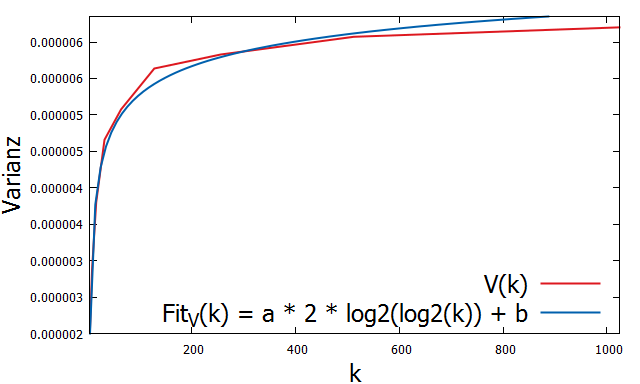
\includegraphics[width=1.2\textwidth]{pictures/min_filter_fit_V_k.png}
    \end{minipage}
    \hspace*{.8cm}
    \begin{minipage}[t]{.30\textwidth}
        \centering
        \raisebox{-0.02cm}{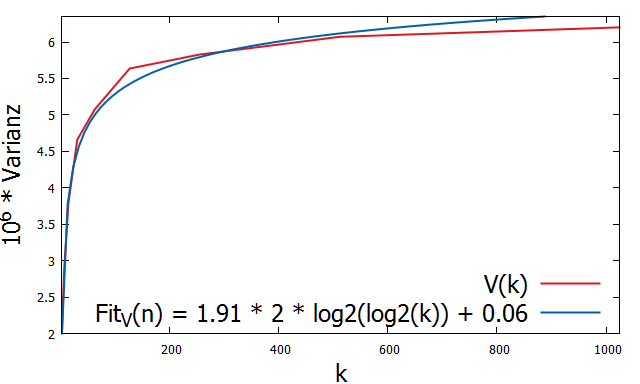
\includegraphics[width=1.21\textwidth]{pictures/min_filter_fit_V_k_loglog.png}}
    \end{minipage}  
    \hspace*{.8cm}
    \begin{minipage}[t]{.30\textwidth}
        \centering
        \raisebox{-0.02cm}{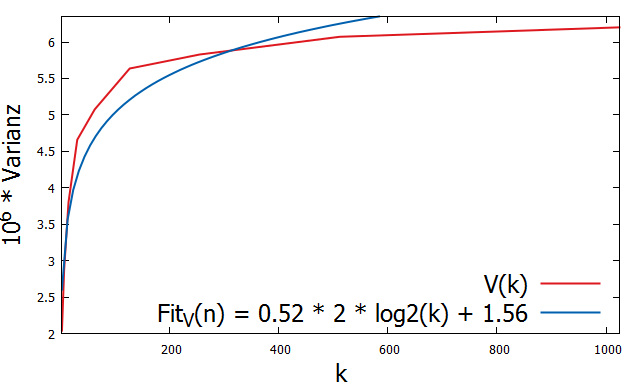
\includegraphics[width=1.21\textwidth]{pictures/min_filter_fit_V_k_log.png}}
    \end{minipage}
    \captionof{figure}{(Skalierter) Fit für $V(k)$ für $\log_2(n)=16$ bezüglich $\log_2(k)$ und $\log_2\log_2(k)$.}\label{fig: min_fit_V_k}
\end{figure}

% ---------------------------------------------------------------
\noindent
Abschließend ist festzuhalten, dass die Güte $\Delta X$ der Filterung einer normalverteilten Zufallsvariable entspricht, deren Erwartungswert von $\sqrt{k}$ und deren Varianz von $1/n$ sowie $\log_2\log_2(k)$ abhängig ist.




%%%%%%%%%%%%%%%%%%%%%%%%%%%%%%%%%%%%%%%%%%%%%%%%%%%%%%%%%%%%%%%%%